\section{Gradient-based correlation coefficient in 3D}\label{sec:uniform-proof}
%%%%%%%%%%%%%%%%%%%%%%%%%%%%%%%%%%%%%%%%%%%%%%%%%%%%%%%%%%%%%%%%%%%%%%%%%%%%%%%%
Assuming we are given two 3D images, denoted as $\I_1$ and $\I_2$, we define $\boldsymbol{G}_{i,x} = \boldsymbol{F}_x \ast \boldsymbol{I}_i$, $\boldsymbol{G}_{i,y} = \boldsymbol{F}_y \ast \boldsymbol{I}_i$, $\boldsymbol{G}_{i,z} = \boldsymbol{F}_z \ast \boldsymbol{I}_i$ as the gradients obtained by convolving $\boldsymbol{I}_i$ with differentiation approximation filters $\boldsymbol{F}_x$, $\boldsymbol{F}_y$ and $\boldsymbol{F}_z$ respectively.  We define a set $P$, which represents the set of indicies corresponding to image support. Given $P$ is of cardinality $N$, we can define $\g_i, i \in \{1,2\}$ as the $N$-dimensional vector obtained by writing $\boldsymbol{G}_i = \boldsymbol{G}_{i,x} + \boldsymbol{G}_{i,y} + \boldsymbol{G}_{i,z}$ in lexicographical order. We can then define the gradient correlation coefficient as
%%%%%%%%%%%%%%%%%%%%%%%%%%%%%%%%%%%%%%%%%%%%%%%%%%%%%%%%%%%%%%%%%%%%%%%%%%%%%%%%
\begin{equation}\label{eq:grad-corr}
    s \triangleq \g_1^T \g_2
\end{equation}
%%%%%%%%%%%%%%%%%%%%%%%%%%%%%%%%%%%%%%%%%%%%%%%%%%%%%%%%%%%%%%%%%%%%%%%%%%%%%%%%

To ensure that the correlation we calculate represents the normal correlations, we suppress the magnitude contribution by using the normalised gradients (i.e normals). We define the normalised gradient as
%%%%%%%%%%%%%%%%%%%%%%%%%%%%%%%%%%%%%%%%%%%%%%%%%%%%%%%%%%%%%%%%%%%%%%%%%%%%%%%%
\begin{equation}\label{eq:tilde-g}
    \tildeg_i = \left[ \tildeg_{i,x} \; \tildeg_{i,y} \; \tildeg_{i,z} \right]^T
\end{equation}
%%%%%%%%%%%%%%%%%%%%%%%%%%%%%%%%%%%%%%%%%%%%%%%%%%%%%%%%%%%%%%%%%%%%%%%%%%%%%%%%
where $\tildeg_{i,x} = \g_{i,x} \, / \, \norm{\g_i}$, $\tildeg_{i,y} = \g_{i,y} \, / \, \norm{\g_i}$ and $\tildeg_{i,z} = \g_{i,z} \, / \, \norm{\g_i}$.

In the following subsections we outline two different angular representations of normals. These angular representations allow us to formulate the correlation as a sum of cosines of gradient orientation.

%%%%%%%%%%%%%%%%%%%%%%%%%%%%%%%%%%%%%%%%%%%%%%%%%%%%%%%%%%%%%%%%%%%%%%%%%%%%%%%%
\subsection{Inner Product Correlation}\label{subsec:inner-product-corr}
%%%%%%%%%%%%%%%%%%%%%%%%%%%%%%%%%%%%%%%%%%%%%%%%%%%%%%%%%%%%%%%%%%%%%%%%%%%%%%%%
The first representation comes in the form of the inner product between the normals of the images. The inner product between the normals is simply defined as $\cos \phi = \tildeg_1 \cdot \tildeg_2$. The inner product within 3D Euclidean space defines the angle between two vectors. Therefore, we can define the correlation coefficient in terms of the inner product as
%%%%%%%%%%%%%%%%%%%%%%%%%%%%%%%%%%%%%%%%%%%%%%%%%%%%%%%%%%%%%%%%%%%%%%%%%%%%%%%%
\begin{equation}\label{eq:inner-product-cosine}
    q_0 \triangleq \sum_{k \in P} \cos [\phi (k)]
\end{equation}
%%%%%%%%%%%%%%%%%%%%%%%%%%%%%%%%%%%%%%%%%%%%%%%%%%%%%%%%%%%%%%%%%%%%%%%%%%%%%%%%

In order for (\ref{eq:inner-product-cosine}) to provide a robust correlation, the visually dissimilar areas must sum to approximately zero. However, claiming robustness using the results of \cite{RefWorks:6} and \cite{RefWorks:68} is not applicable in the case of (\ref{eq:inner-product-cosine}). Nevertheless, we can demonstrate the robustness of (\ref{eq:inner-product-cosine}) by studying the statistical properties of $\cos[\phi (k)]$ (instead of the angles as in \cite{RefWorks:6, RefWorks:68}). As can be seen in Figure~\ref{fig:dot-product-distribution}, the inner product of the normalised gradients resembles a Laplace distribution, where the Laplacian is given by
%%%%%%%%%%%%%%%%%%%%%%%%%%%%%%%%%%%%%%%%%%%%%%%%%%%%%%%%%%%%%%%%%%%%%%%%%%%%%%%%
\begin{equation}\label{eq:laplace-distribution}
    L(x \mid 0, b) = \frac{1}{2b} \exp \left\{ - \frac{\abs{x}}{b} \right\}
\end{equation}
%%%%%%%%%%%%%%%%%%%%%%%%%%%%%%%%%%%%%%%%%%%%%%%%%%%%%%%%%%%%%%%%%%%%%%%%%%%%%%%%
Hence,
%%%%%%%%%%%%%%%%%%%%%%%%%%%%%%%%%%%%%%%%%%%%%%%%%%%%%%%%%%%%%%%%%%%%%%%%%%%%%%%%
\begin{equation}\label{eq:laplace-approx-zero}
    q_0 \approx \mathbb{E} \left( L(\cos[\phi (k)] \mid 0, b) \right) \approx 0
\end{equation}
%%%%%%%%%%%%%%%%%%%%%%%%%%%%%%%%%%%%%%%%%%%%%%%%%%%%%%%%%%%%%%%%%%%%%%%%%%%%%%%%
where $\mathbb{E}$ is the expectation operator. Through experimentation we have found that the inner product often approximates a zero-mean Laplace distribution and so it is still valid to assume that
%%%%%%%%%%%%%%%%%%%%%%%%%%%%%%%%%%%%%%%%%%%%%%%%%%%%%%%%%%%%%%%%%%%%%%%%%%%%%%%%
\begin{equation}\label{eq:inner-product-approx-zero}
    q_0 = \sum_{k \in P} \cos [\phi (k)] \simeq 0
\end{equation}
%%%%%%%%%%%%%%%%%%%%%%%%%%%%%%%%%%%%%%%%%%%%%%%%%%%%%%%%%%%%%%%%%%%%%%%%%%%%%%%%
%%%%%%%%%%%%%%%%%%%%%%%%%%%%%%%%%%%%%%%%%%%%%%%%%%%%%%%%%%%%%%%%%%%%%%%%%%%%%%%%
\begin{figure}[h!]
        \centering
        \begin{subfigure}[b]{0.22\textwidth}
                \centering
                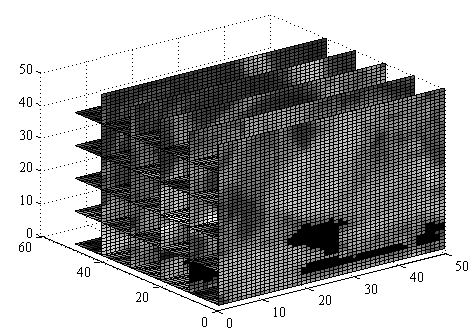
\includegraphics[width=\textwidth]{images/dot_product_image1}
                \subcaption{}
                \label{fig:dot-product-image1}
        \end{subfigure}
        \begin{subfigure}[b]{0.22\textwidth}
                \centering
                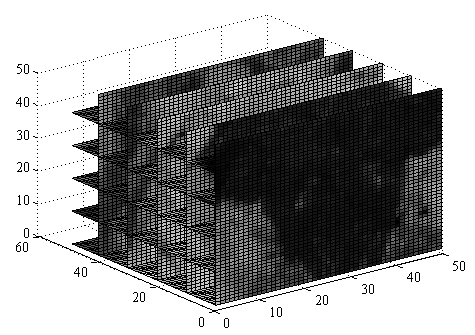
\includegraphics[width=\textwidth]{images/dot_product_image2}
                \subcaption{}
                \label{fig:dot-product-image2}
        \end{subfigure}
        \\ % New Line
        \begin{subfigure}[b]{0.45\textwidth}
                \centering
                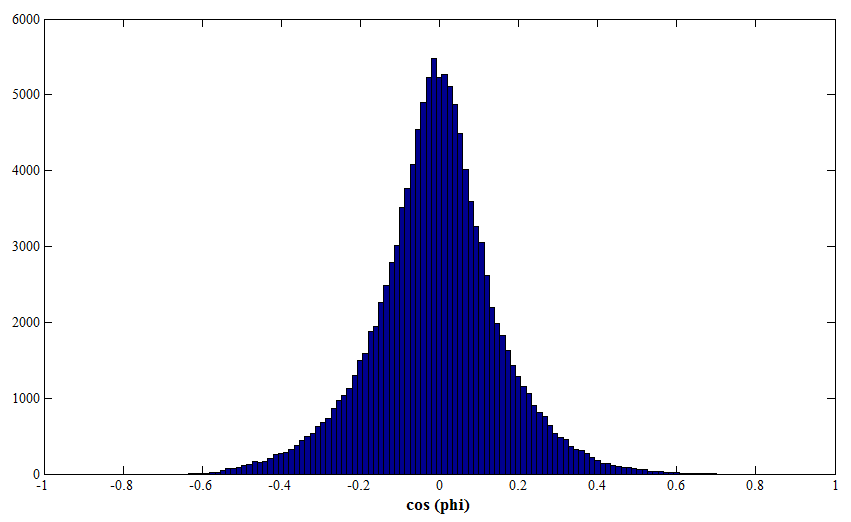
\includegraphics[width=\textwidth]{images/dot_product_hist}
                \subcaption{}
                \label{fig:dot-product-hist}
        \end{subfigure}
        \caption{(a)-(b) Two images use to compare the dot product distribution. The images are visually dissimilar and taken from the Visible Human data-set. The volumes are represented as a series of 2D slices. (c) The distribution of $\cos \phi$ between the two images.}
        \label{fig:dot-product-distribution}
\end{figure}
%%%%%%%%%%%%%%%%%%%%%%%%%%%%%%%%%%%%%%%%%%%%%%%%%%%%%%%%%%%%%%%%%%%%%%%%%%%%%%%%

%%%%%%%%%%%%%%%%%%%%%%%%%%%%%%%%%%%%%%%%%%%%%%%%%%%%%%%%%%%%%%%%%%%%%%%%%%%%%%%%
\subsection{Spherical Correlation}\label{subsec:spherical-corr}
%%%%%%%%%%%%%%%%%%%%%%%%%%%%%%%%%%%%%%%%%%%%%%%%%%%%%%%%%%%%%%%%%%%%%%%%%%%%%%%%
In order to use the robustness properties of \cite{RefWorks:6}, we apply the spherical representation of normals. This allows us to represent the normals in terms of their azimuth and elevation angle. Due to the normalised nature of our gradients, every coordinate lies upon the surface of a unit sphere. The spherical representation is defined by the azimuth angle, $\phi_i \triangleq \arctan [\frac{\tildeg_{i,y}}{\tildeg_{i,x}}]$ and the elevation angle, $\theta_i \triangleq \arccos [\tildeg_{i,z}]$. We can then formulate the correlation as a sum of angle differences
%%%%%%%%%%%%%%%%%%%%%%%%%%%%%%%%%%%%%%%%%%%%%%%%%%%%%%%%%%%%%%%%%%%%%%%%%%%%%%%%
\begin{equation}\label{eq:spherical-cosine}
    s \triangleq \sum_{k \in P} \cos [\Delta \phi (k)] + \sum_{k \in P} \cos [\Delta \theta (k)]
\end{equation}
%%%%%%%%%%%%%%%%%%%%%%%%%%%%%%%%%%%%%%%%%%%%%%%%%%%%%%%%%%%%%%%%%%%%%%%%%%%%%%%%
where $\Delta \phi (k) \triangleq \phi_1 (k) - \phi_2 (k)$ and $\Delta \theta (k) \triangleq \theta_1 (k) - \theta_2 (k)$.

$\phi_i$ is equivalent to gradient orientation in 2D images \cite{RefWorks:6}, hence the difference $\Delta \phi (k)$ between two visually pixel-wise dissimilar images can be assumed to follow $U(0, 2 \pi)$. This was also widely validated in the 3D case through extensive experimentation. Figure~\ref{fig:spherical-distribution} shows the approximate uniform distribution formed by $\Delta \phi$ data from within the Visible Human data set.
%%%%%%%%%%%%%%%%%%%%%%%%%%%%%%%%%%%%%%%%%%%%%%%%%%%%%%%%%%%%%%%%%%%%%%%%%%%%%%%%
\begin{figure}[h!]
        \centering
        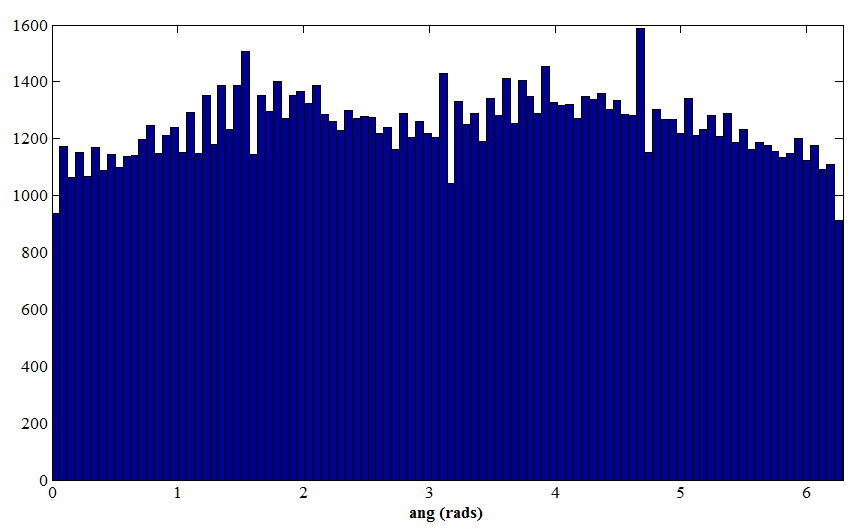
\includegraphics[width=0.45\textwidth]{images/spherical_hist}
        \caption{The distribution of $\Delta \phi$ for the images shown in Figures \ref{fig:dot-product-image1} and \ref{fig:dot-product-image2}}
        \label{fig:spherical-distribution}
\end{figure}
%%%%%%%%%%%%%%%%%%%%%%%%%%%%%%%%%%%%%%%%%%%%%%%%%%%%%%%%%%%%%%%%%%%%%%%%%%%%%%%%

Unfortunately, we cannot apply directly the optimisation procedure proposed in \cite{RefWorks:6} to optimise (\ref{eq:spherical-cosine}) with regards to the parameters, since it is based on the sum of two different cost functions. Nevertheless, we can formulate (\ref{eq:spherical-cosine}) as a least-squares problem, by observing that, since $\cos^2 \alpha + \sin^2 \alpha = 1 \; \forall \alpha$, then maximisation of
%%%%%%%%%%%%%%%%%%%%%%%%%%%%%%%%%%%%%%%%%%%%%%%%%%%%%%%%%%%%%%%%%%%%%%%%%%%%%%%%
\begin{equation}\label{eq:maximise-cos}
   \sum_{k \in P} \cos [\Delta \phi (k)] + \sum_{k \in P} \cos [\Delta \theta (k)]
\end{equation}
%%%%%%%%%%%%%%%%%%%%%%%%%%%%%%%%%%%%%%%%%%%%%%%%%%%%%%%%%%%%%%%%%%%%%%%%%%%%%%%%
is equivalent to the minimisation of
%%%%%%%%%%%%%%%%%%%%%%%%%%%%%%%%%%%%%%%%%%%%%%%%%%%%%%%%%%%%%%%%%%%%%%%%%%%%%%%%
\begin{equation}\label{eq:minimise-least-squares}
       \sum_{k \in P} \Big[ 
        \begin{pmatrix}
            \cos \phi_1 (k) \\ 
            \sin \phi_1 (k) \\
            \cos \theta_1 (k) \\ 
            \sin \theta_1 (k)
        \end{pmatrix}
        -
        \begin{pmatrix}
            \cos \phi_2 (k) \\ 
            \sin \phi_2 (k) \\
            \cos \theta_2 (k) \\ 
            \sin \theta_2 (k)
        \end{pmatrix}
        \Big] ^2
\end{equation}
%%%%%%%%%%%%%%%%%%%%%%%%%%%%%%%%%%%%%%%%%%%%%%%%%%%%%%%%%%%%%%%%%%%%%%%%%%%%%%%%
This least-squares formulation of the correlation can then be easily solved within any least-squares minimisation framework. 

%%%%%%%%%%%%%%%%%%%%%%%%%%%%%%%%%%%%%%%%%%%%%%%%%%%%%%%%%%%%%%%%%%%%%%%%%%%%%%%%
\subsection{Parametric Image Alignment}\label{subsec:parametric-alignment}
%%%%%%%%%%%%%%%%%%%%%%%%%%%%%%%%%%%%%%%%%%%%%%%%%%%%%%%%%%%%%%%%%%%%%%%%%%%%%%%%
Parametric image alignment assumes that $\I_1$ and $\I_2$ are related by a parametric warp
%%%%%%%%%%%%%%%%%%%%%%%%%%%%%%%%%%%%%%%%%%%%%%%%%%%%%%%%%%%%%%%%%%%%%%%%%%%%%%%%
\begin{equation}\label{eq:image-warp}
   I_1 (\boldsymbol{x_k}) = I_2(\W(\boldsymbol{x_k};\p)), \; \forall{k} \in P
\end{equation}
%%%%%%%%%%%%%%%%%%%%%%%%%%%%%%%%%%%%%%%%%%%%%%%%%%%%%%%%%%%%%%%%%%%%%%%%%%%%%%%%
where $\W(\boldsymbol{x_k};\p)$ is a parametric transformation with respect to the unknown parameters $\p = \left[p(1), ..., p(n)\right]^T$ and the image coordinates $\boldsymbol{x_k} = \left[x_1(k) x_2(k)\right]^T$. We can then estimate $\p$ by minimizing an objective function in an iterative fashion by performing a Taylor expansion on either $\I_1$ or $\I_2$. In the following two sections we will show how to optimise (\ref{eq:inner-product-cosine}) and (\ref{eq:spherical-cosine}) with respect to the unknown motion parameters, $\p$.